%======================================================================
\NEWSEC
%======================================================================

\subsection{\ssInstallEnzop}

%----------------------------------------------------------------------
\begin{frame}[fragile,label=ss-install-enzop] 
\secframetitle{\ssInstallEnzop}
\framesubtitle{Enzo-P source code: \url{https://bitbucket.org/cello-project}}
\footnotesize \enzopcello\ source is available from \textcolor{green!50!black}{\url{https://bitbucket.org/cello-project}}
\begin{center}
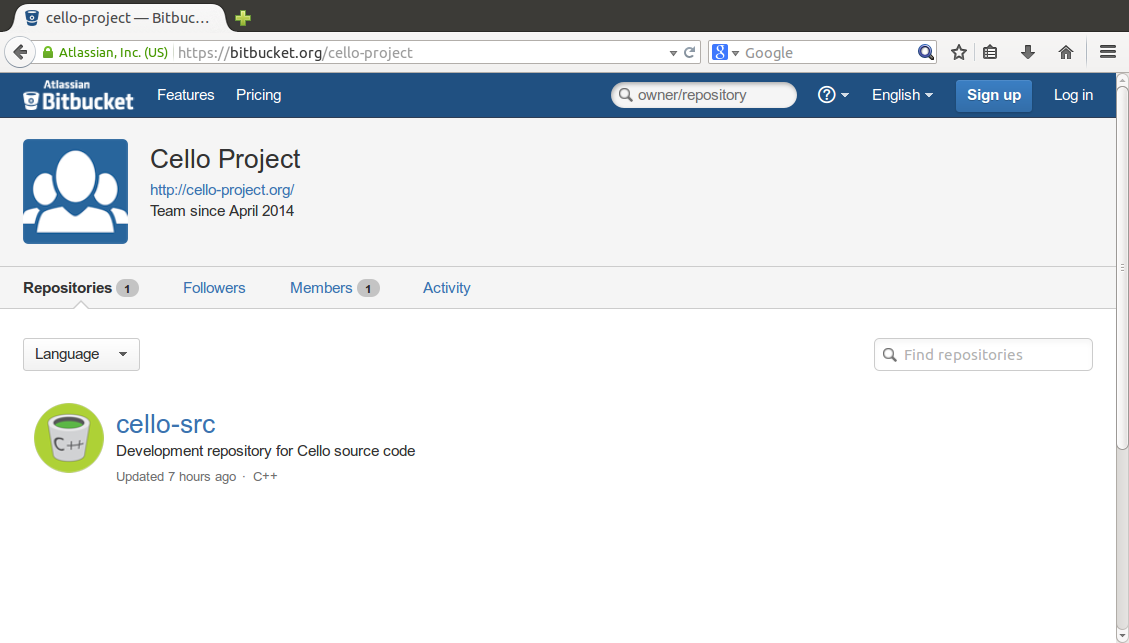
\includegraphics[width=4.00in]{cello-download.png}
\end{center}
\end{frame}
\setbeamercolor{monitor-2.png}{bg=RGB{43,43,51}}

%----------------------------------------------------------------------
\begin{frame}[fragile] 
\secframetitle{\ssInstallEnzop}
\framesubtitle{Downloading Enzo-P/Cello}
\footnotesize
\begin{semiverbatim}
 \prompt\ \redcode{hg clone https://bitbucket.org/cello-project/cello-src}\cursor{1}  
 \uncover<2->{destination directory: cello-src}
 \uncover<2->{requesting all changes}
 \uncover<2->{adding changesets} 
 \uncover<2->{adding manifests} 
 \uncover<2->{adding file changes} 
 \uncover<2->{added 3529 changesets with 21657 changes to 4353 files (+1 heads)} 
 \uncover<2->{updating to branch default} 
 \uncover<2->{resolving manifests} 
 \uncover<2->{\vdots}
 \uncover<2->{getting scons-LICENSE}
 \uncover<2->{getting scons-README}
 \uncover<2->{getting scons-local-2.2.0/SCons/Action.py}
 \uncover<2->{924 files updated, 0 files merged, 0 files removed, 0 files unresolved}
\end{semiverbatim}
\end{frame}

